% !TeX root = ../../thesis.tex
\chapter{Mesh quality plots}\label{ch:appendix}

This appendix aims to visualize some mesh quality metrics for various 3D mesh geometries used throughout the current thesis. The mesh quality plots show the uniformity of generated meshes considering the applied refinement on the biodegradation interface.

\section{Mesh quality metrics}

In finite element simulations, the accuracy and reliability of results are heavily dependent on the quality of the mesh. Mesh quality metrics are therefore used to assess the quality of the mesh before analysis. Some common metrics used to evaluate the quality of a mesh include aspect ratio, skewness, orthogonality, and element size. Aspect ratio measures the ratio of the longest side of an element to the shortest side, while skewness measures the deviation of the element from an ideal shape. Orthogonality measures the angle between adjacent element faces, and element size measures the minimum size of the element. A good mesh should have well-shaped elements, minimal skewness and distortion, and uniform element size distribution.

For measuring the quality of various 3D meshes in the current thesis, two metrics were selected to be measured: Gamma index and aspect ratio, both plotted versus the number of elements sharing the same metric value. The Gamma value, calculated using GMSH, is obtained by dividing the inscribed radius of each element to it circumscribed radius. In GMSH, it is calculated by dividing the volume of each element to the sum of the area of its faces, multiplied by the maximum edge length. 

Aspect ratio measures the ratio of the longest edge of an element to the shortest edge length and is used to assess the distortion of the element. A high aspect ratio indicates that the element is highly distorted and can cause inaccurate results or numerical instability in the simulation. In contrast, a low aspect ratio indicates a more regular shape and a better representation of the geometry being simulated. Generally, a good mesh should have elements with an aspect ratio as close to one as possible, which indicates that the elements are well-shaped and do not deviate significantly from their ideal geometries. 

The aspect ratio measurements were done using the SALOME platform. For a  tetrahedral element shown in Fig. \ref{fig:appendix_tetrahedral}, the aspect ratio is calculated as:
\begin{equation}
Q=\frac{h_{\max }}{2 \sqrt{6} r},
\end{equation}
in which $h_{\max}$ is the maximum edge length ($h_{\max }=\max \left(h_{a b}, h_{a c}, h_{a d}, h_{b c}, h_{b d}, h_{c d}\right)$), and $r$ is the inradius of the tetrahedron, which can be calculated as follows: 
\begin{equation}
r=\frac{|\alpha|}{\left\|N_{\{a, b, c\}}\right\|+\left\|N_{\{a, b, d\}}\right\|+\left\|N_{\{a, c, d\}}\right\|+\left\|N_{\{b, c, d\}}\right\|},
\end{equation} 
where $N_{\{a, b, c\}}$ is a normal vector to the face defined by vertices $\{a, b, c\}$. $\alpha$ and $N$ can be calculated as follows:
\begin{equation}
\alpha=\overrightarrow{a b} \cdot(\overrightarrow{a c} \times \overrightarrow{a d}) \quad N_{\{a, b, c\}}=\overrightarrow{a b} \times \overrightarrow{a c}.
\end{equation}


\begin{figure}[h]
\centering
\medskip
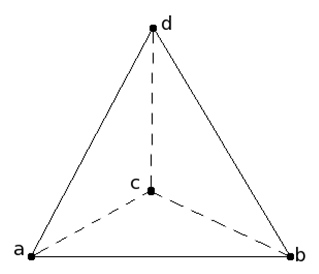
\includegraphics[width=0.4\textwidth]{tetrahedral.png}
\caption[A simple tetrahedral element for demonstrating aspect ratio calculation]{A simple tetrahedral element for demonstrating aspect ratio calculation.} \label{fig:appendix_tetrahedral}
\end{figure}


\section{Mesh used for the core computational model}

Fig \ref{fig:appendix_narrow_cuboid} shows the quality plots for the mesh used in the narrow cuboid model in Chapter \ref{ch:core} for validating the model, containing $\num{18049471}$ elements. Similarly, Fig \ref{fig:appendix_screw} shows the quality plots for the screw mesh used as a sample case study, containing $\num{1440439}$ elements.

\begin{figure}[!h]
\centering
\medskip
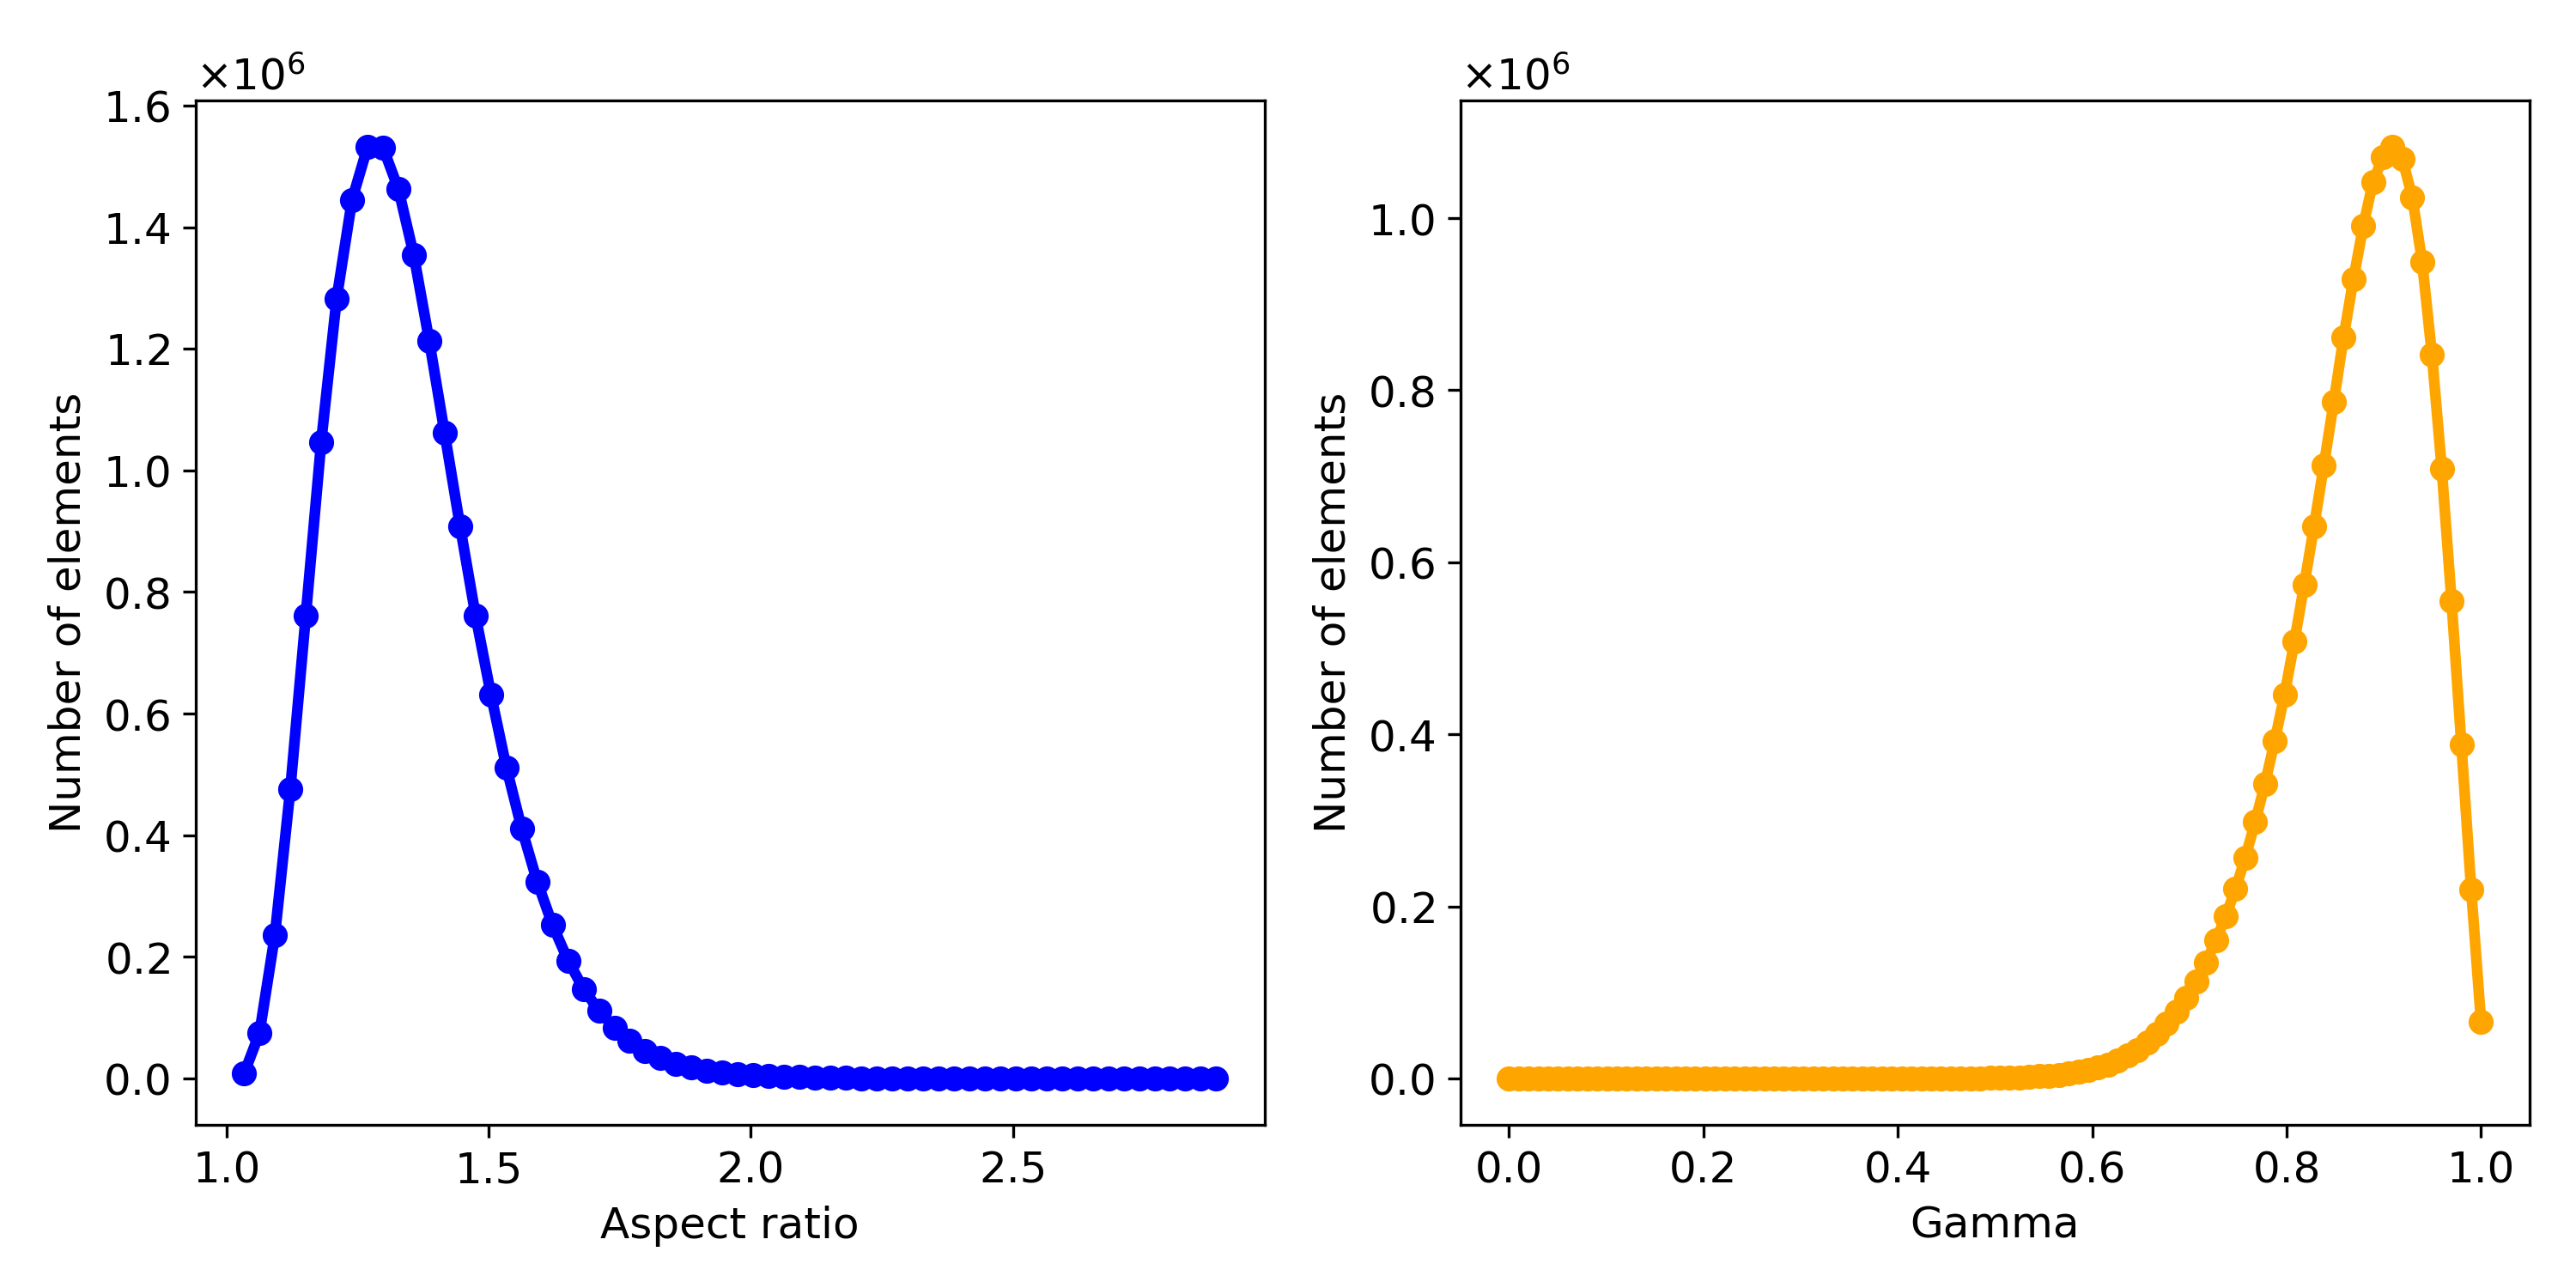
\includegraphics[width=\textwidth]{narrow_cuboid_quality.png}
\caption[Mesh quality plots for the narrow cuboid model]{Mesh quality plots for the narrow cuboid model (Fig. \ref{fig:simulation_setup}).} \label{fig:appendix_narrow_cuboid}
\end{figure}

\begin{figure}[!h]
\centering
\medskip
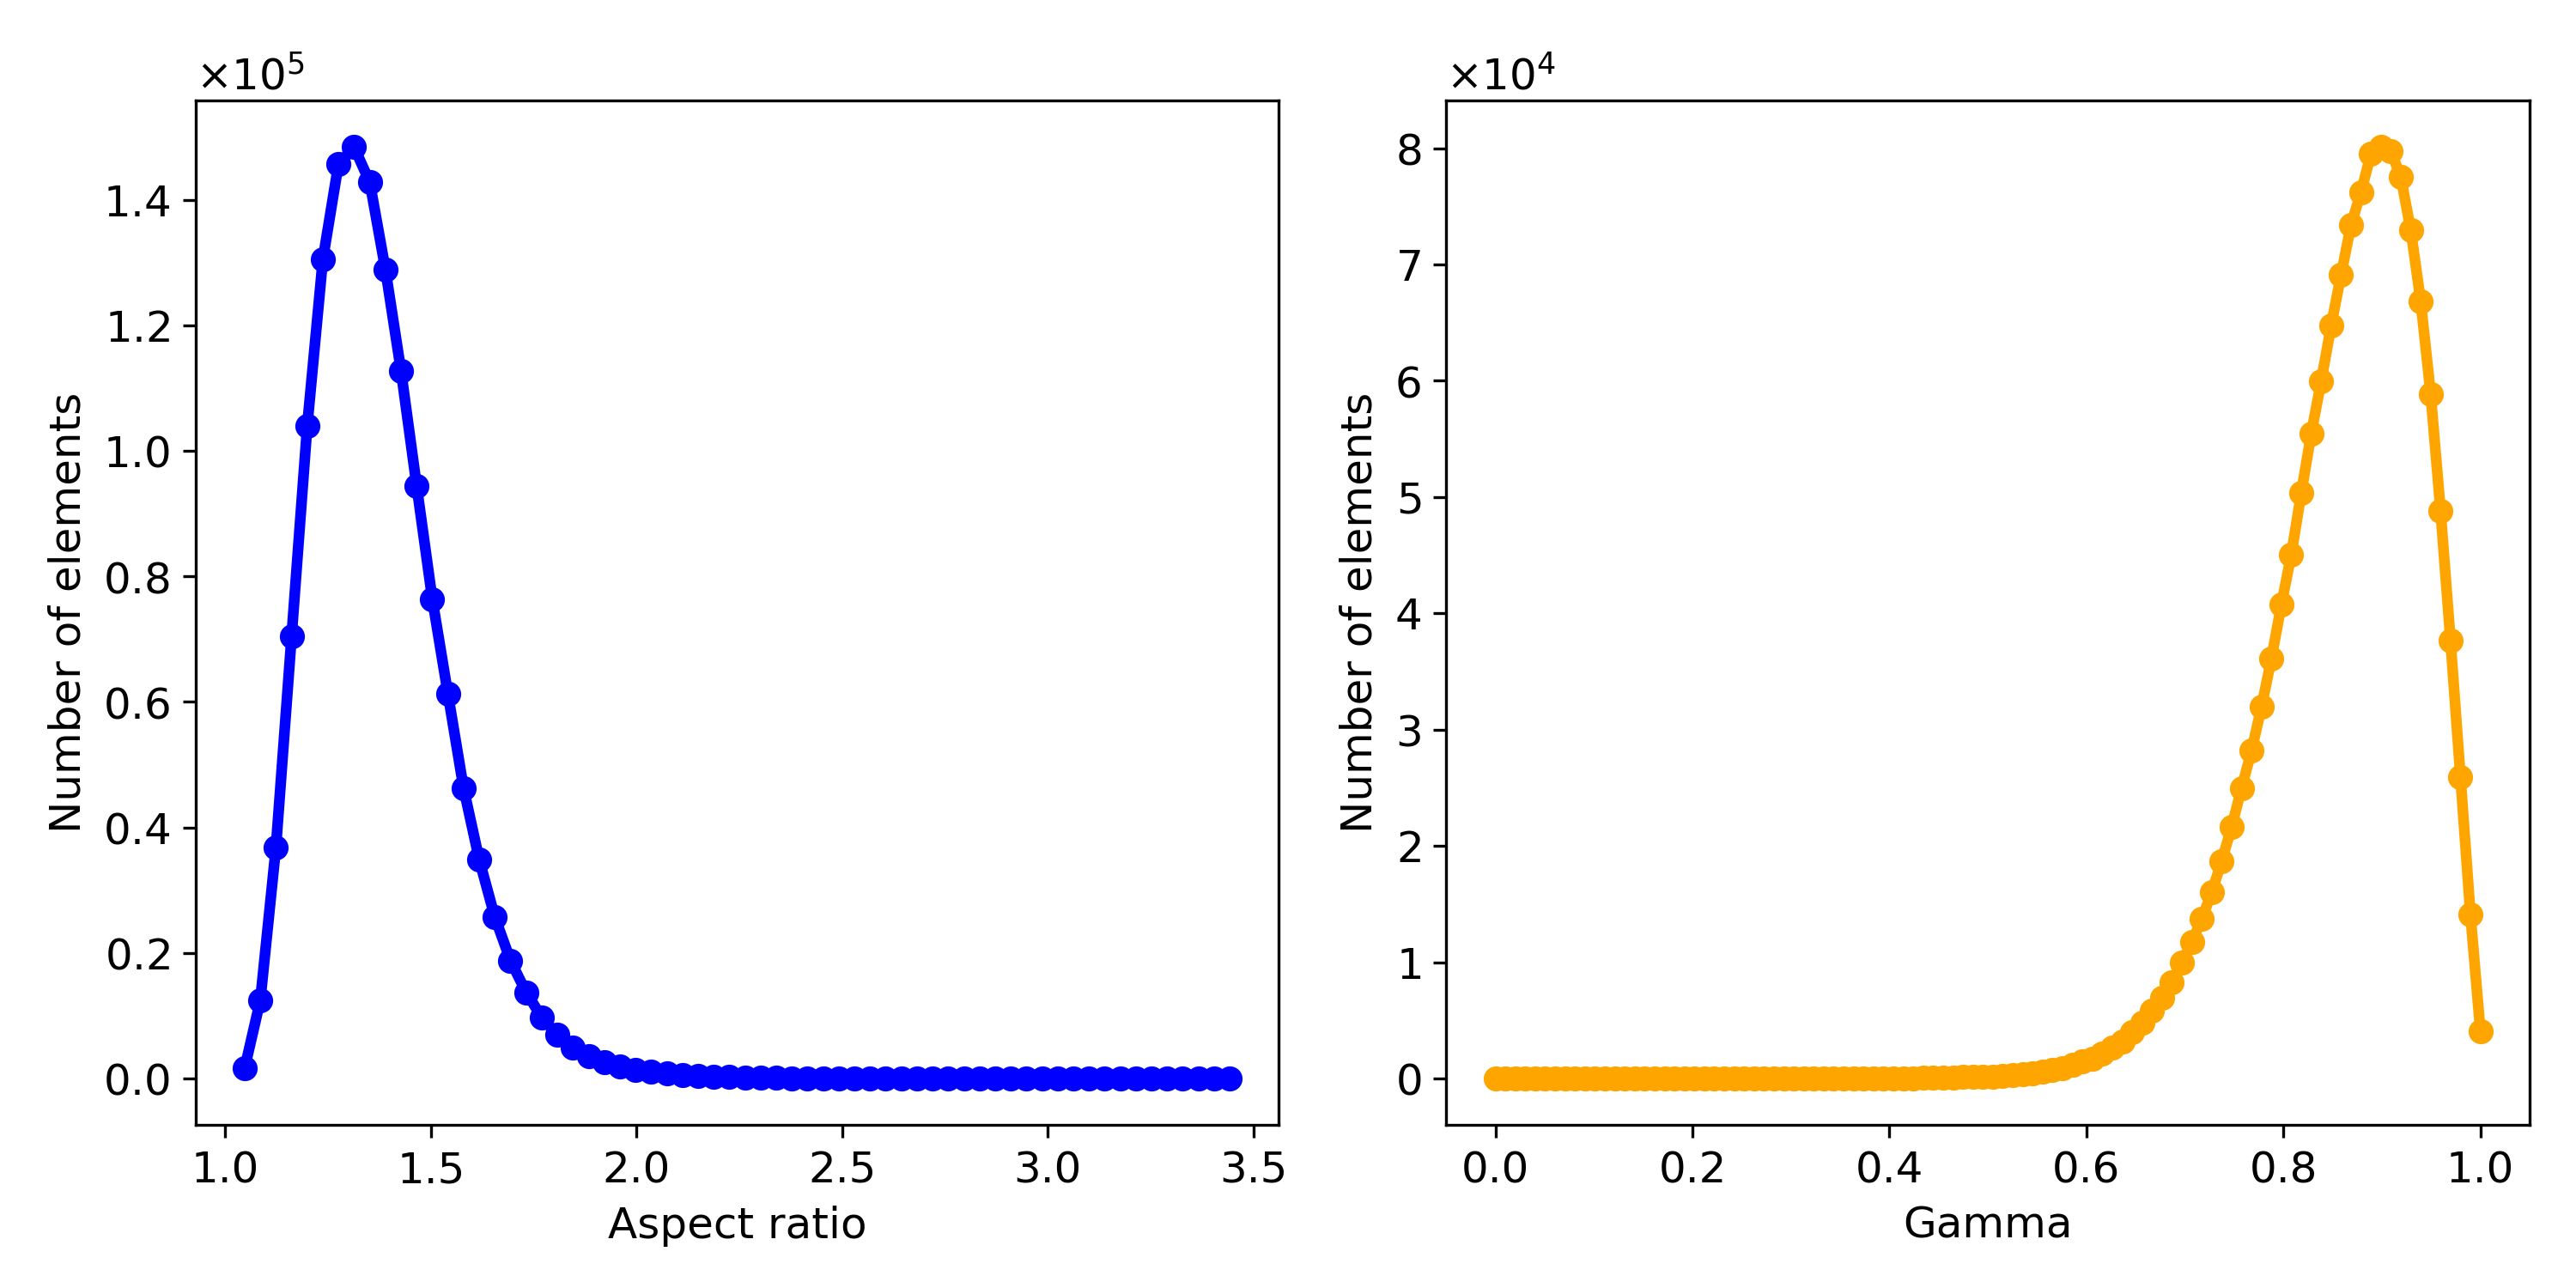
\includegraphics[width=\textwidth]{screw_quality.png}
\caption[Mesh quality plots for the screw model]{Mesh quality plots for the screw model (Fig. \ref{fig:results_screw}).} \label{fig:appendix_screw}
\end{figure}


\section{Mesh used for the extended model}

Fig \ref{fig:appendix_kinetics} shows the quality plots for the mesh used in the chamber setup for the extended model in Chapter \ref{ch:kinetics}, containing $\num{290997}$ elements.

\begin{figure}[!h]
\centering
\medskip
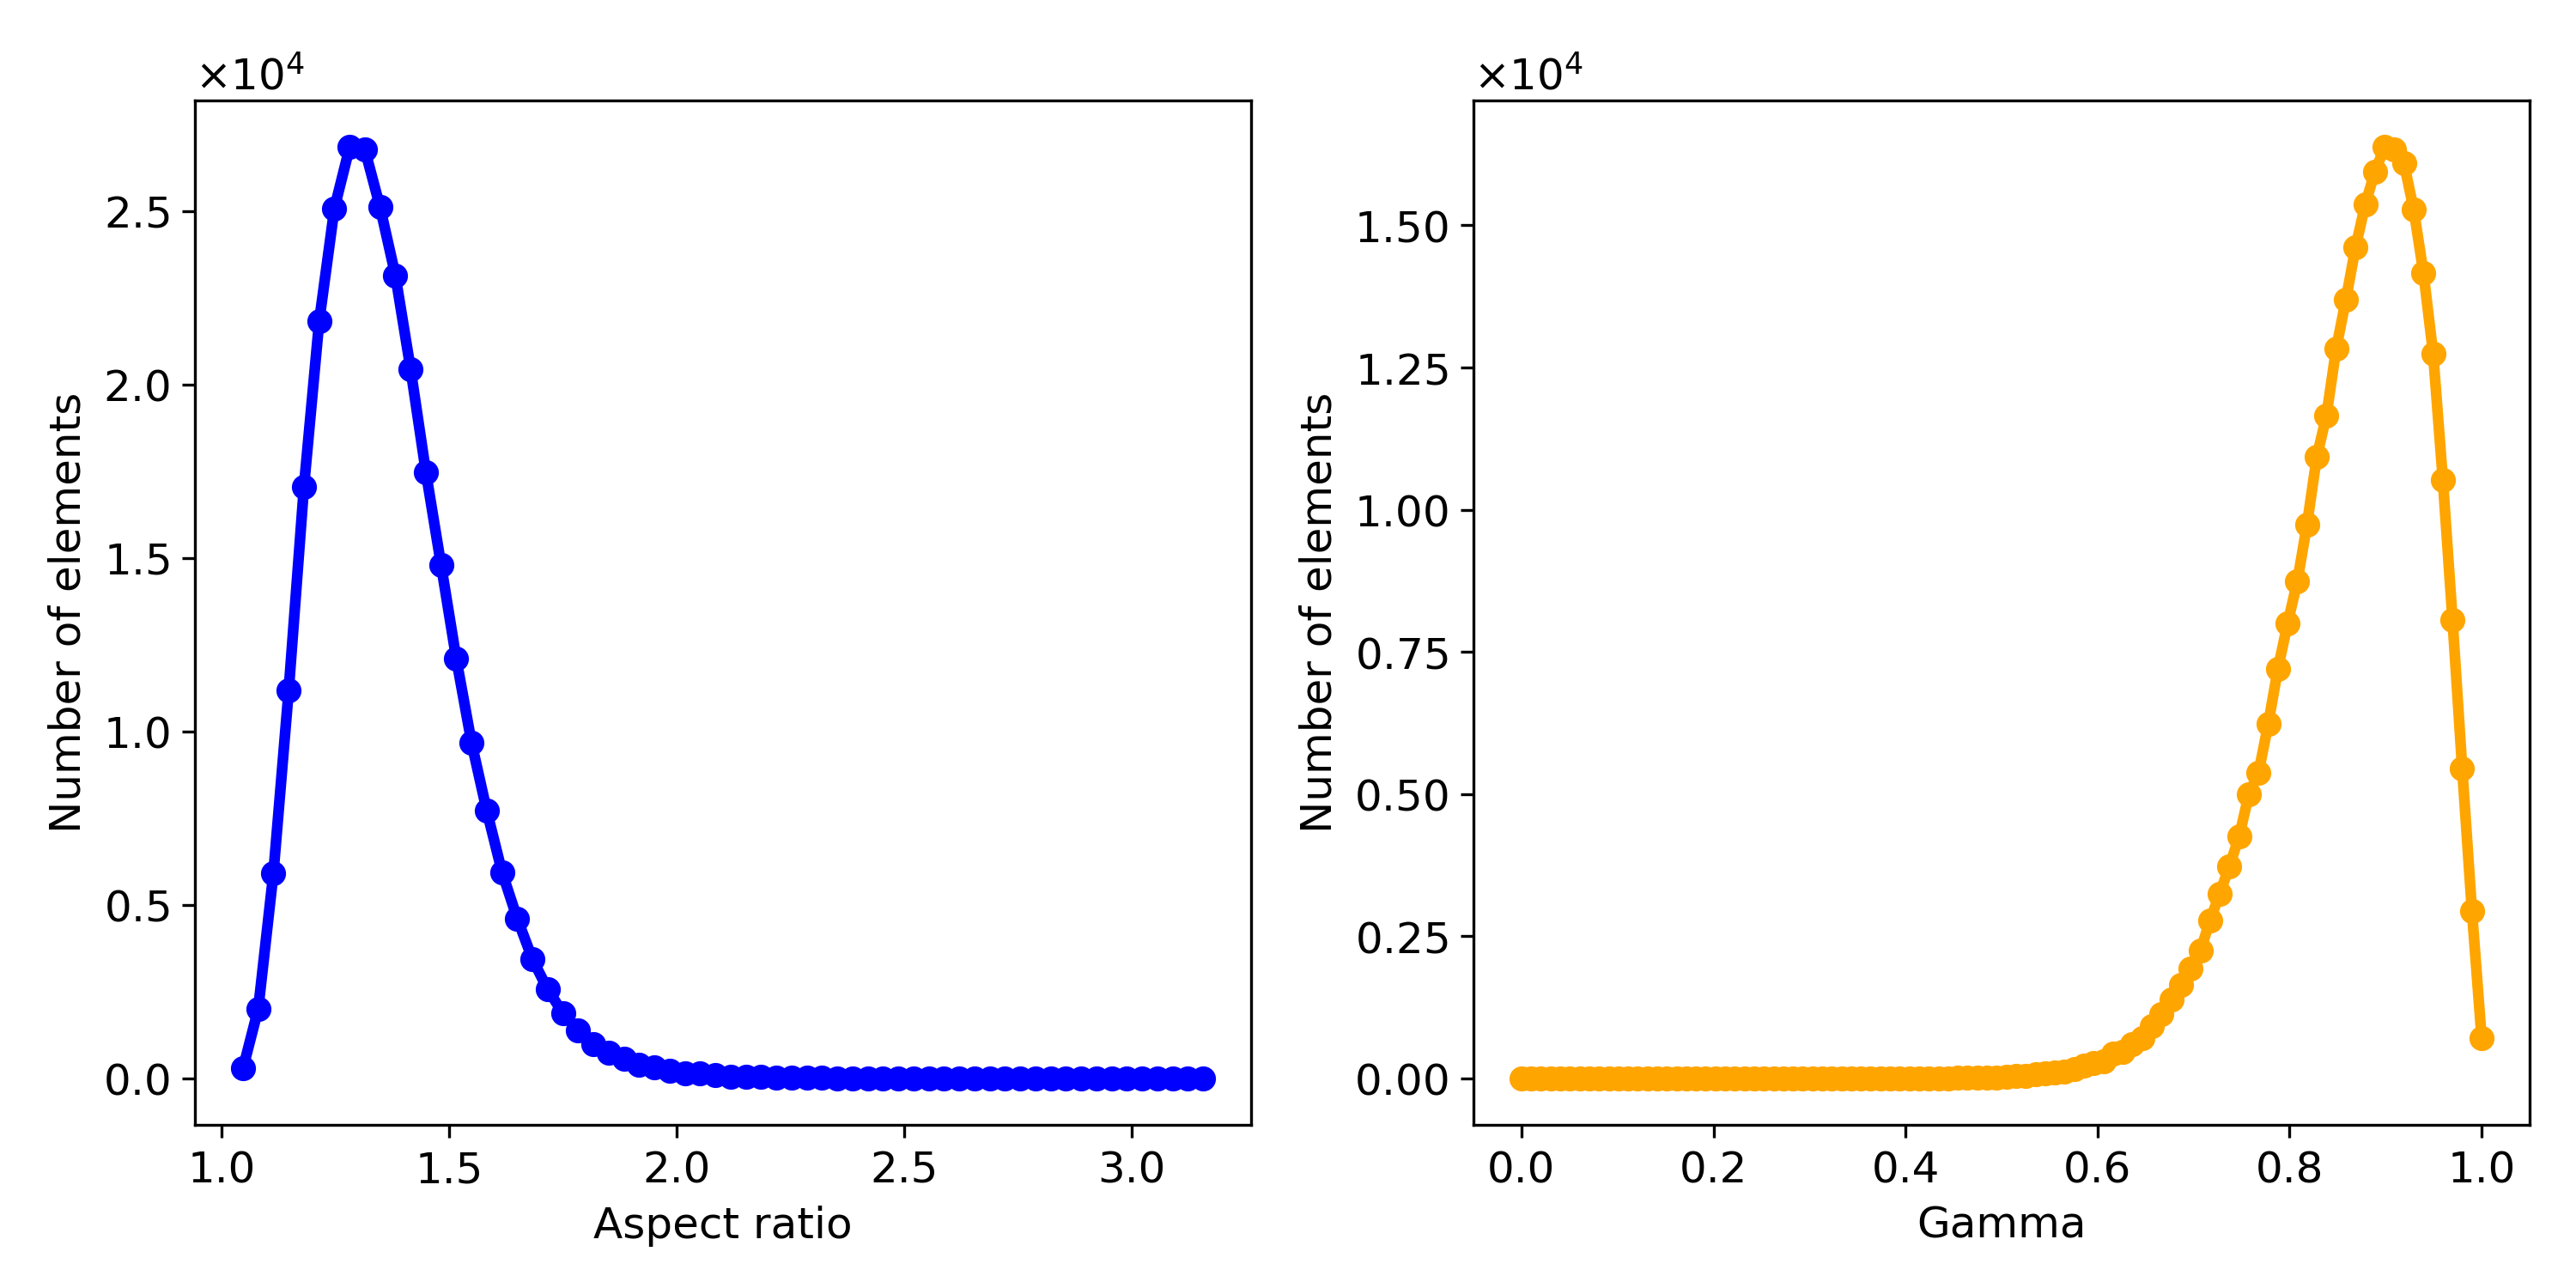
\includegraphics[width=\textwidth]{kinetics_quality.png}
\caption[Mesh quality plots for the local pH model]{Mesh quality plots for the local pH model (Fig. \ref{fig:kinetics_model_setup}).} \label{fig:appendix_kinetics}
\end{figure}

\section{Mesh used for the performance analysis model}

Fig \ref{fig:appendix_cuboid} shows the quality plots for the mesh used for the biodegradation simulations performed in Chapter \ref{ch:hpc}, containing $\num{830808}$ elements.

\begin{figure}[!h]
\centering
\medskip
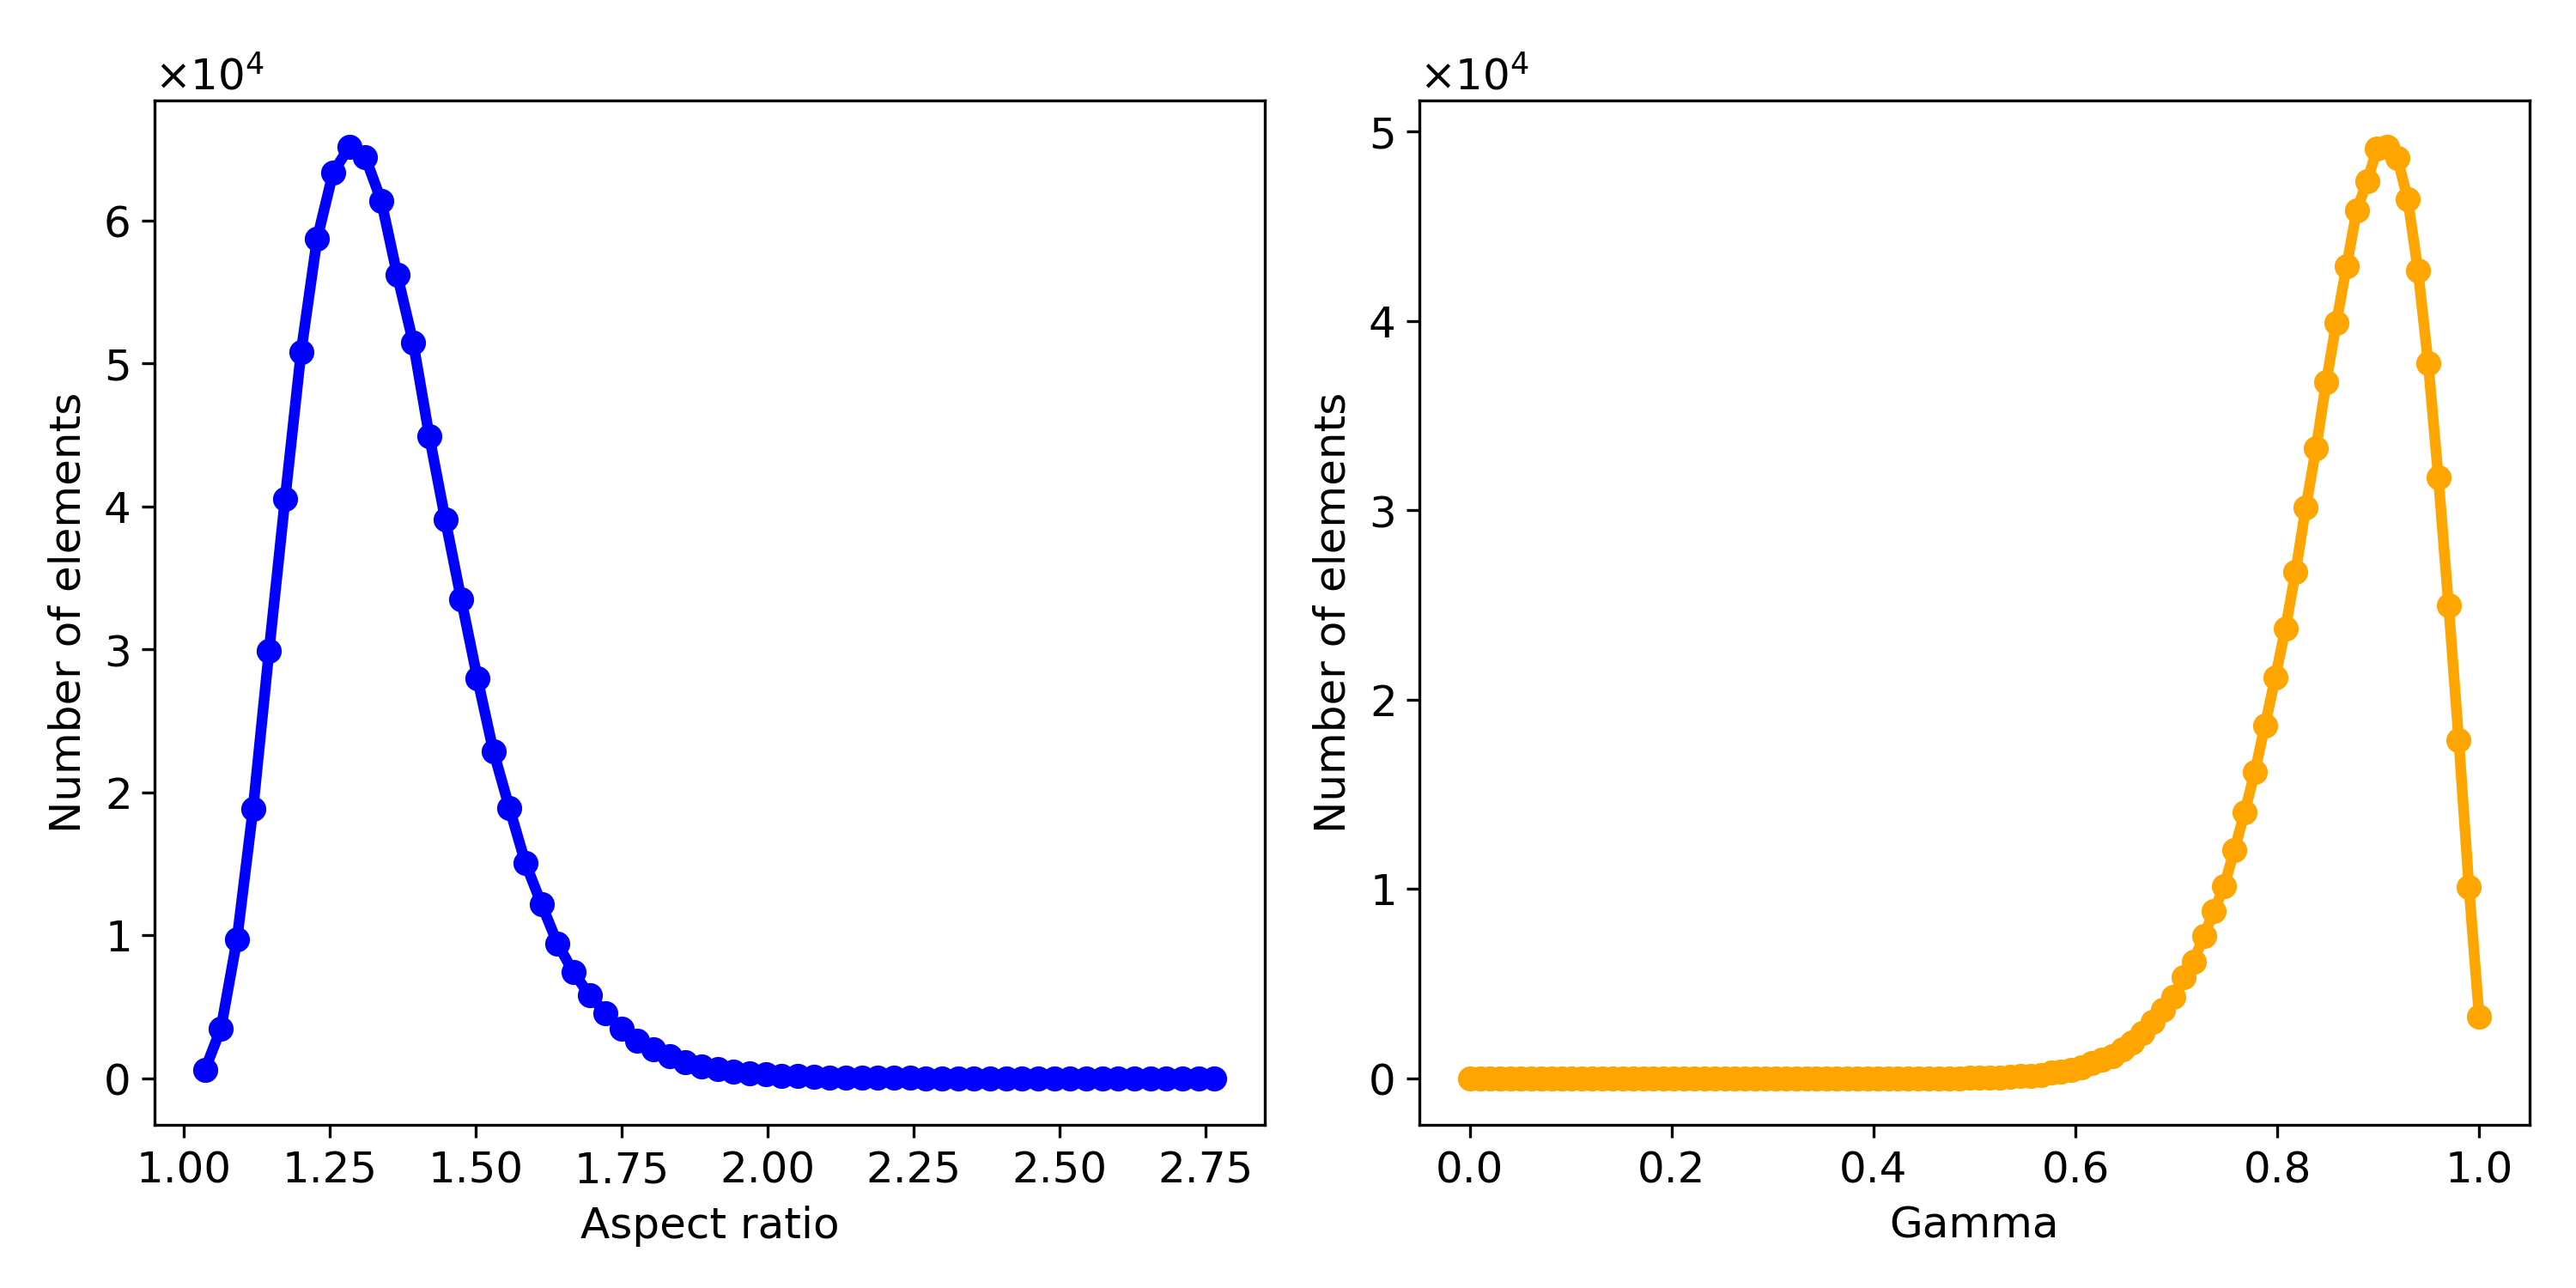
\includegraphics[width=\textwidth]{cuboid_quality.png}
\caption[Mesh quality plots for the cubic block model]{Mesh quality plots for the cubic block model (Fig. \ref{fig:simulation_setup_parallel}).} \label{fig:appendix_cuboid}
\end{figure}

\section{Mesh used for the acetabular implant model}

Fig \ref{fig:appendix_cup} shows the quality plots for the mesh used for the acetabular cup model in Chapter \ref{ch:cup}, containing $\num{45870053}$ elements.

\begin{figure}[!h]
\centering
\medskip
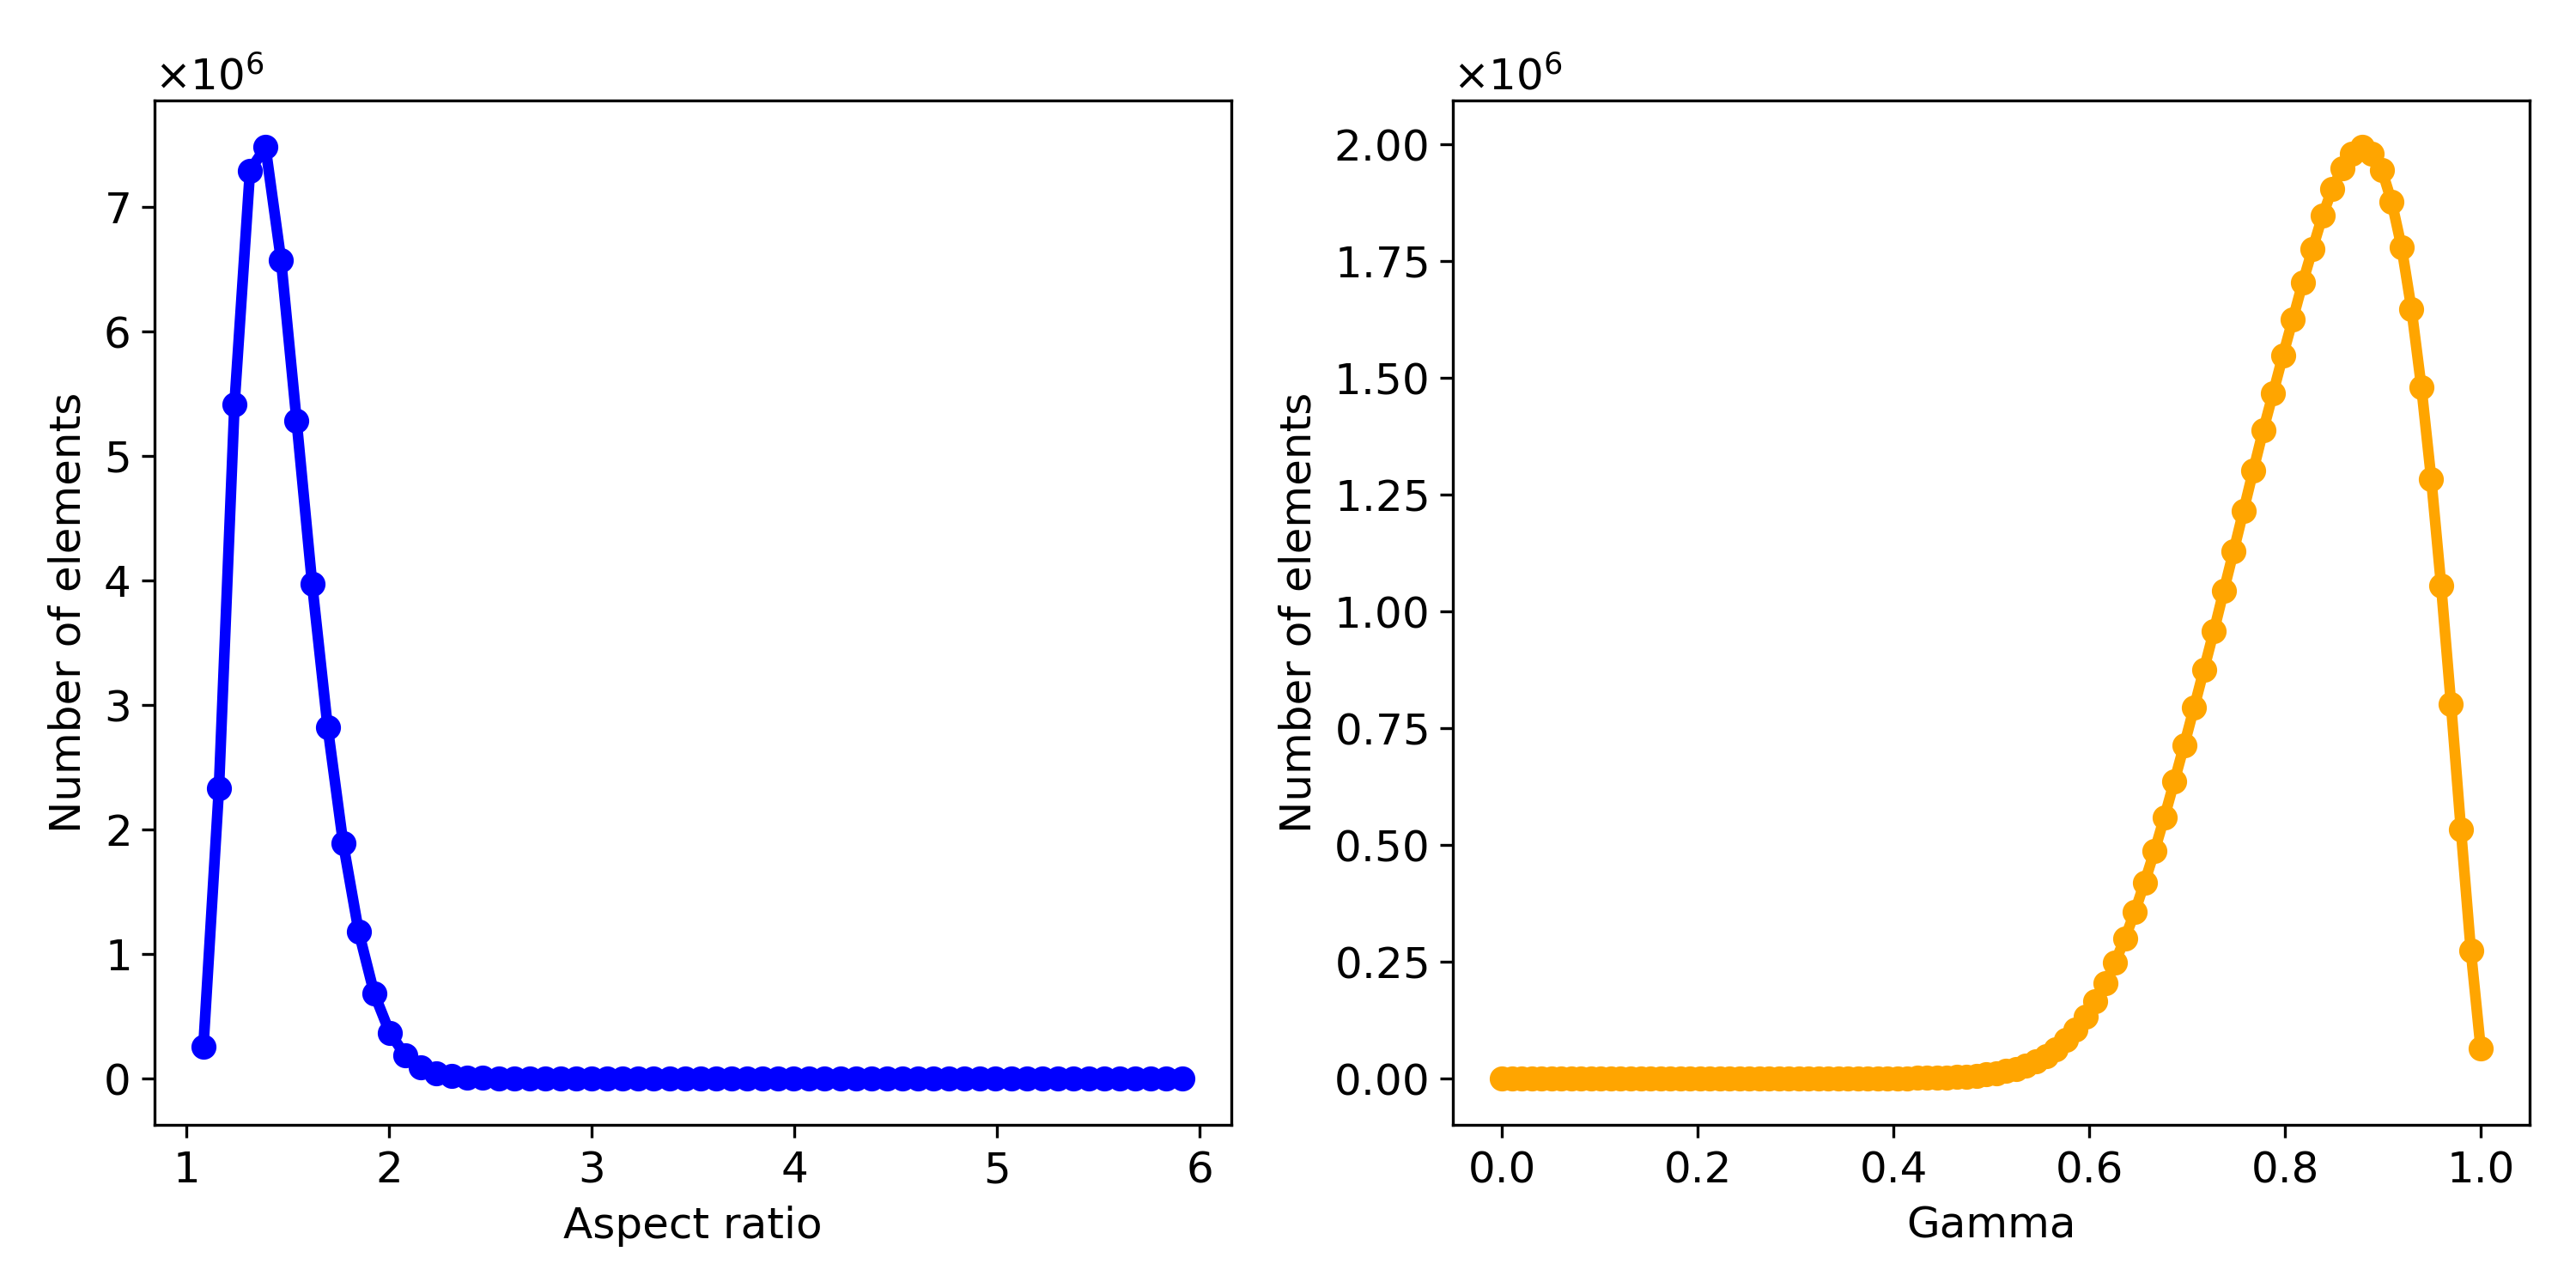
\includegraphics[width=\textwidth]{cup_quality.png}
\caption[Mesh quality plots for the patient-specific acetabular implant model]{Mesh quality plots for the patient-specific acetabular implant model (Fig. \ref{fig:cup_model}).} \label{fig:appendix_cup}
\end{figure}

\section{Mesh used for the mandibular implant model}

Fig \ref{fig:appendix_mandible} shows the quality plots for the mesh used for the mandibular plate model in Chapter \ref{ch:mandible}, containing $\num{19924153}$ elements.

\begin{figure}[!h]
\centering
\medskip
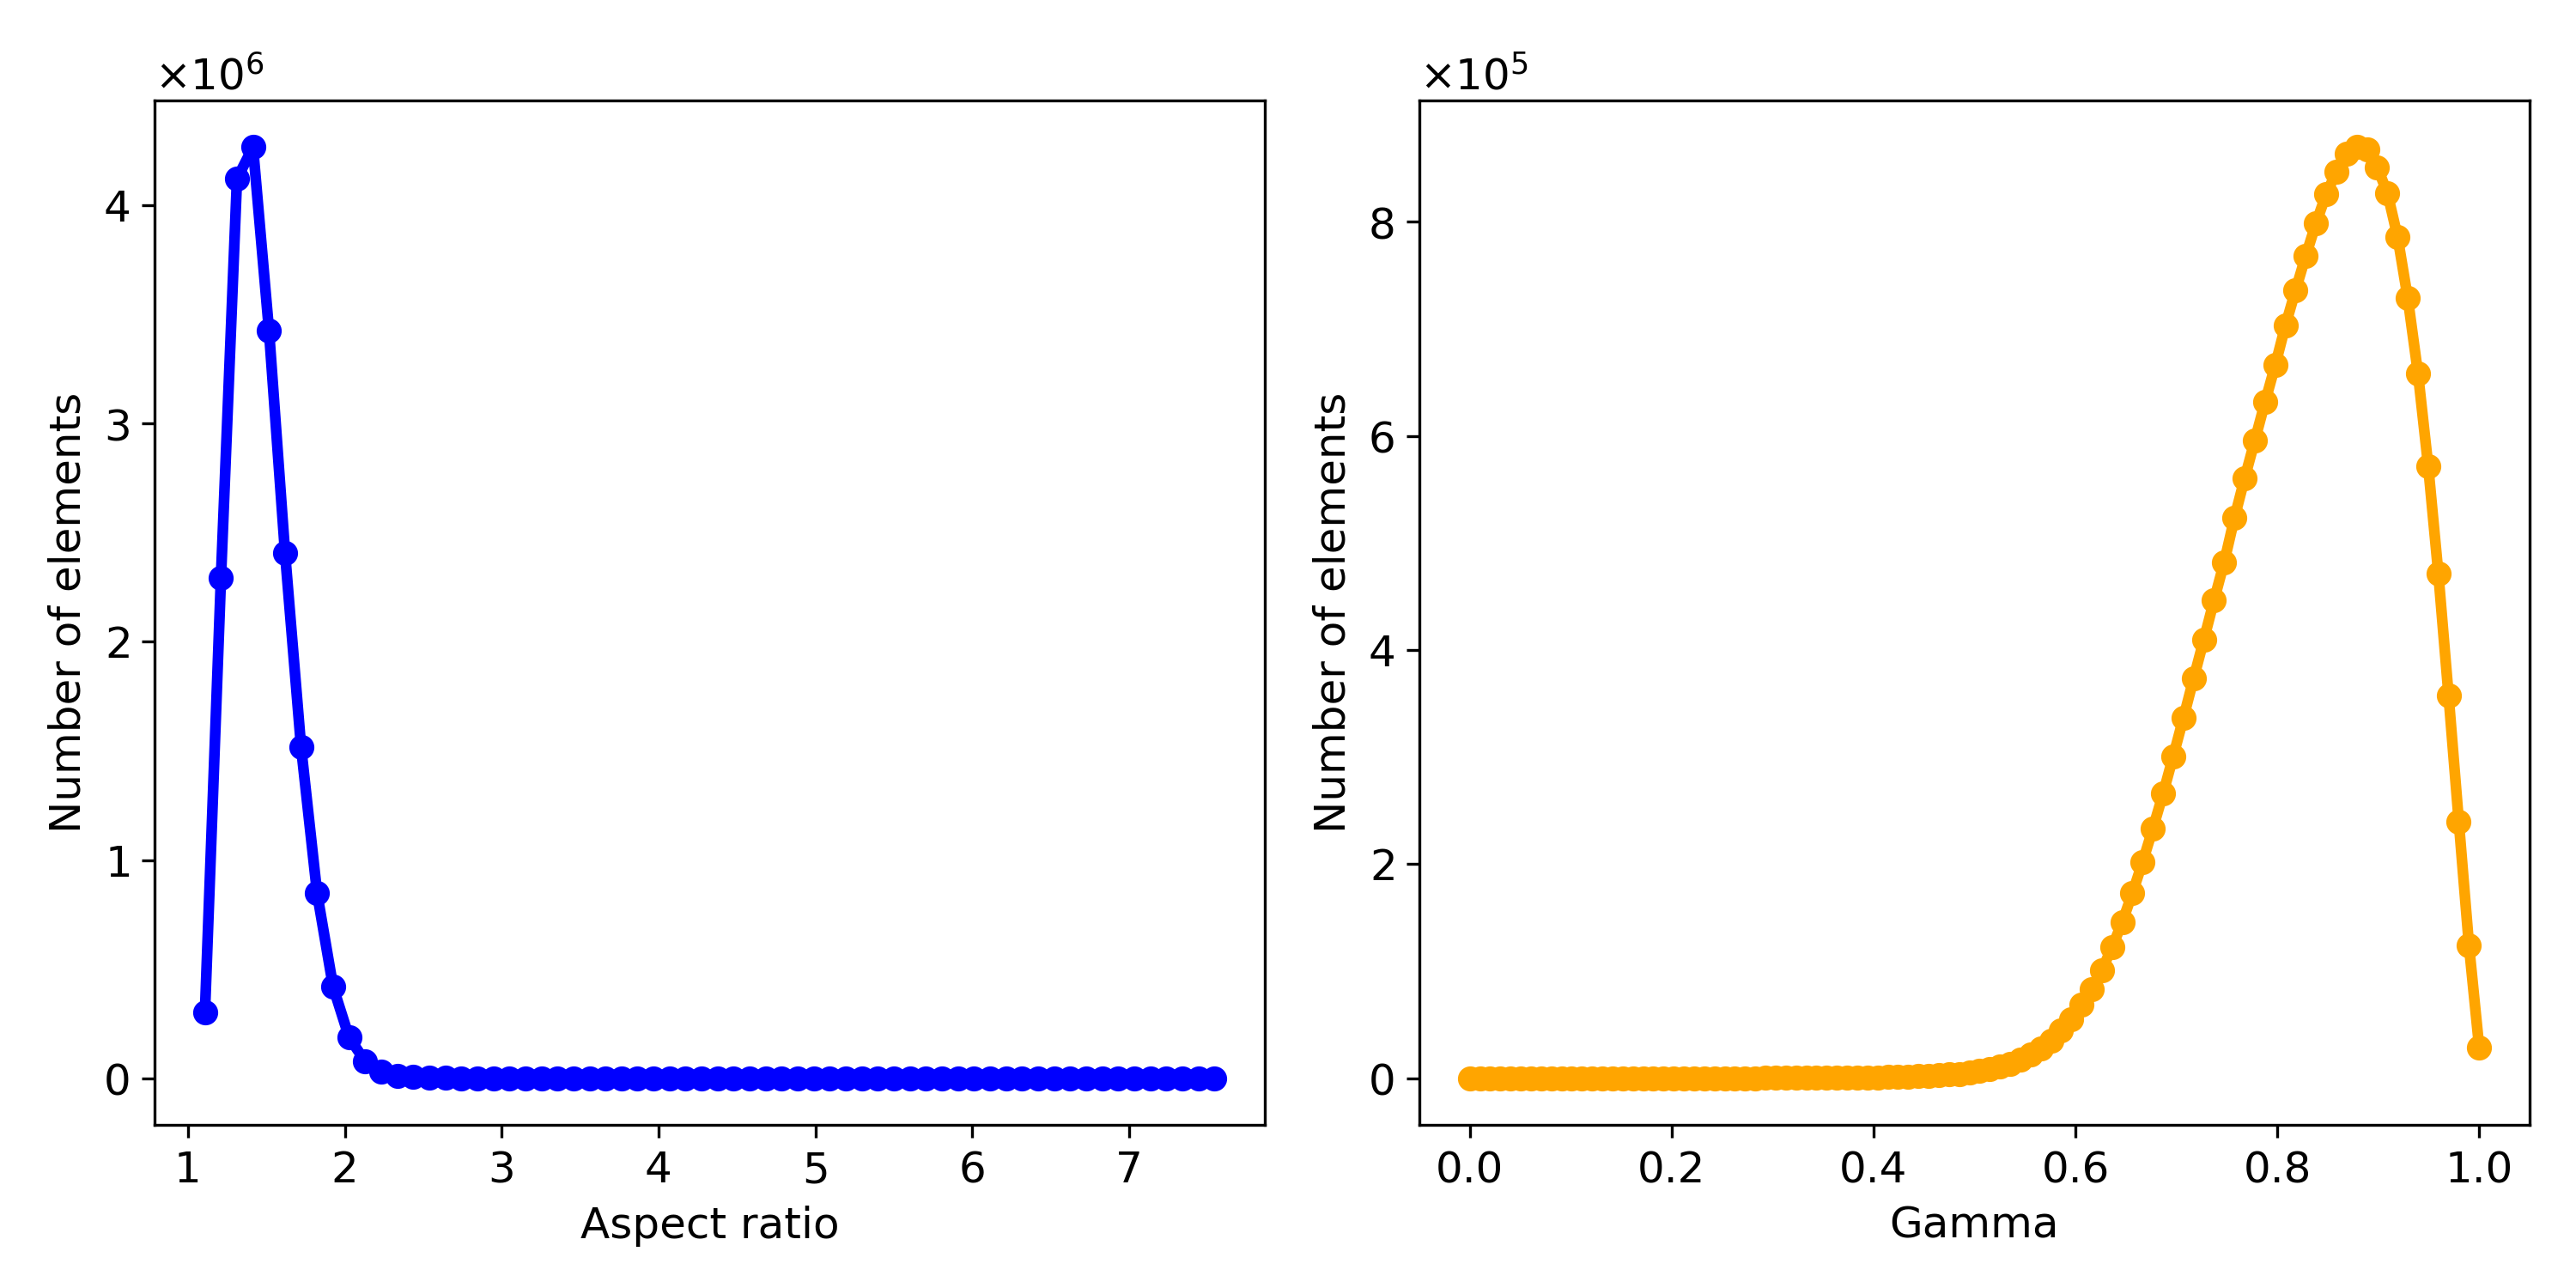
\includegraphics[width=\textwidth]{mandible_quality.png}
\caption[Mesh quality plots for the mandibular implant model]{Mesh quality plots for the mandibular implant model (Fig. \ref{fig:results_degradation}).} \label{fig:appendix_mandible}
\end{figure}

%%%%%%%%%%%%%%%%%%%%%%%%%%%%%%%%%%%%%%%%%%%%%%%%%%
% Keep the following \cleardoublepage at the end of this file, 
% otherwise \includeonly includes empty pages.
\cleardoublepage

